\chapter{\label{cap:avances}Avances}

Los avances que se han realizado en relación a mi proyecto son los siguientes.

\section{\label{sec:bobinasBombeoOptico}Bobinas del bombeo óptico}

Como ya mencioné, con el fin de compensar el campo magnético terrestre a la vez de generar el campo para romper la degeneración de los niveles Zeeman, necesitamos bobinas alrededor de los experimentos.

La compensación del campo terrestre se hace con tres pares de bobinas, su diseño estuvo a cargo de un compañero del laboratorio. Un par de bobinas se alinean de manera que compartan el mismo eje axial, la corriente eléctrica que se suministra se manda para que circule en la misma dirección en ambas bobinas, si la separación entre éstas es similar a algún tamaño característico de una bobina (por ejemplo, el radio en bobinas circulares) entonces el campo magnético alrededor del eje axial y entre ambas bobinas es constante, lo que se denomina como \emph{configuración de Helmholtz}. Con el uso de tres pares de bobinas en dicha configuración, y dispuestas de tal forma que sus ejes axiales sean ortogonales entre sí, podemos tener un campo magnético constante en una dirección arbitraria deseada y compensar así el campo de la Tierra. En la figura~\ref{fig:bobinasBombeoOptico} se muestran estas bobinas.

\p Aunque la construcción y montaje de las bobinas ya está realizado, no las hemos calibrado para compensar el campo terrestre, nos falta un circuito electrónico para modificar la corriente en las bobinas rápido entre mediciones experimentales. El técnico académico del laboratorio ya se encarga de su elaboración. Aún así, hemos aprovechado estas bobinas para modificar el campo cuadrupolar necesario para la trampa MOT: debido a los desperfectos experimentales como la alineación de la optomecánica o el lugar donde están colocadas las bobinas de la MOT, el centro del campo cuadrupolar no está necesariamente alineado con el centro de la zona que define el cruce de los tres brazos de luz de la MOT, como consecuencia la temperatura de los átomos en la MOT incrementa debido al desbalance de fuerzas.

\newsavebox{\bobinasBox}
\begin{figure}[!ht]
\centering
\begin{minipage}{0.8\textwidth}
\centering
\sbox{\bobinasBox}{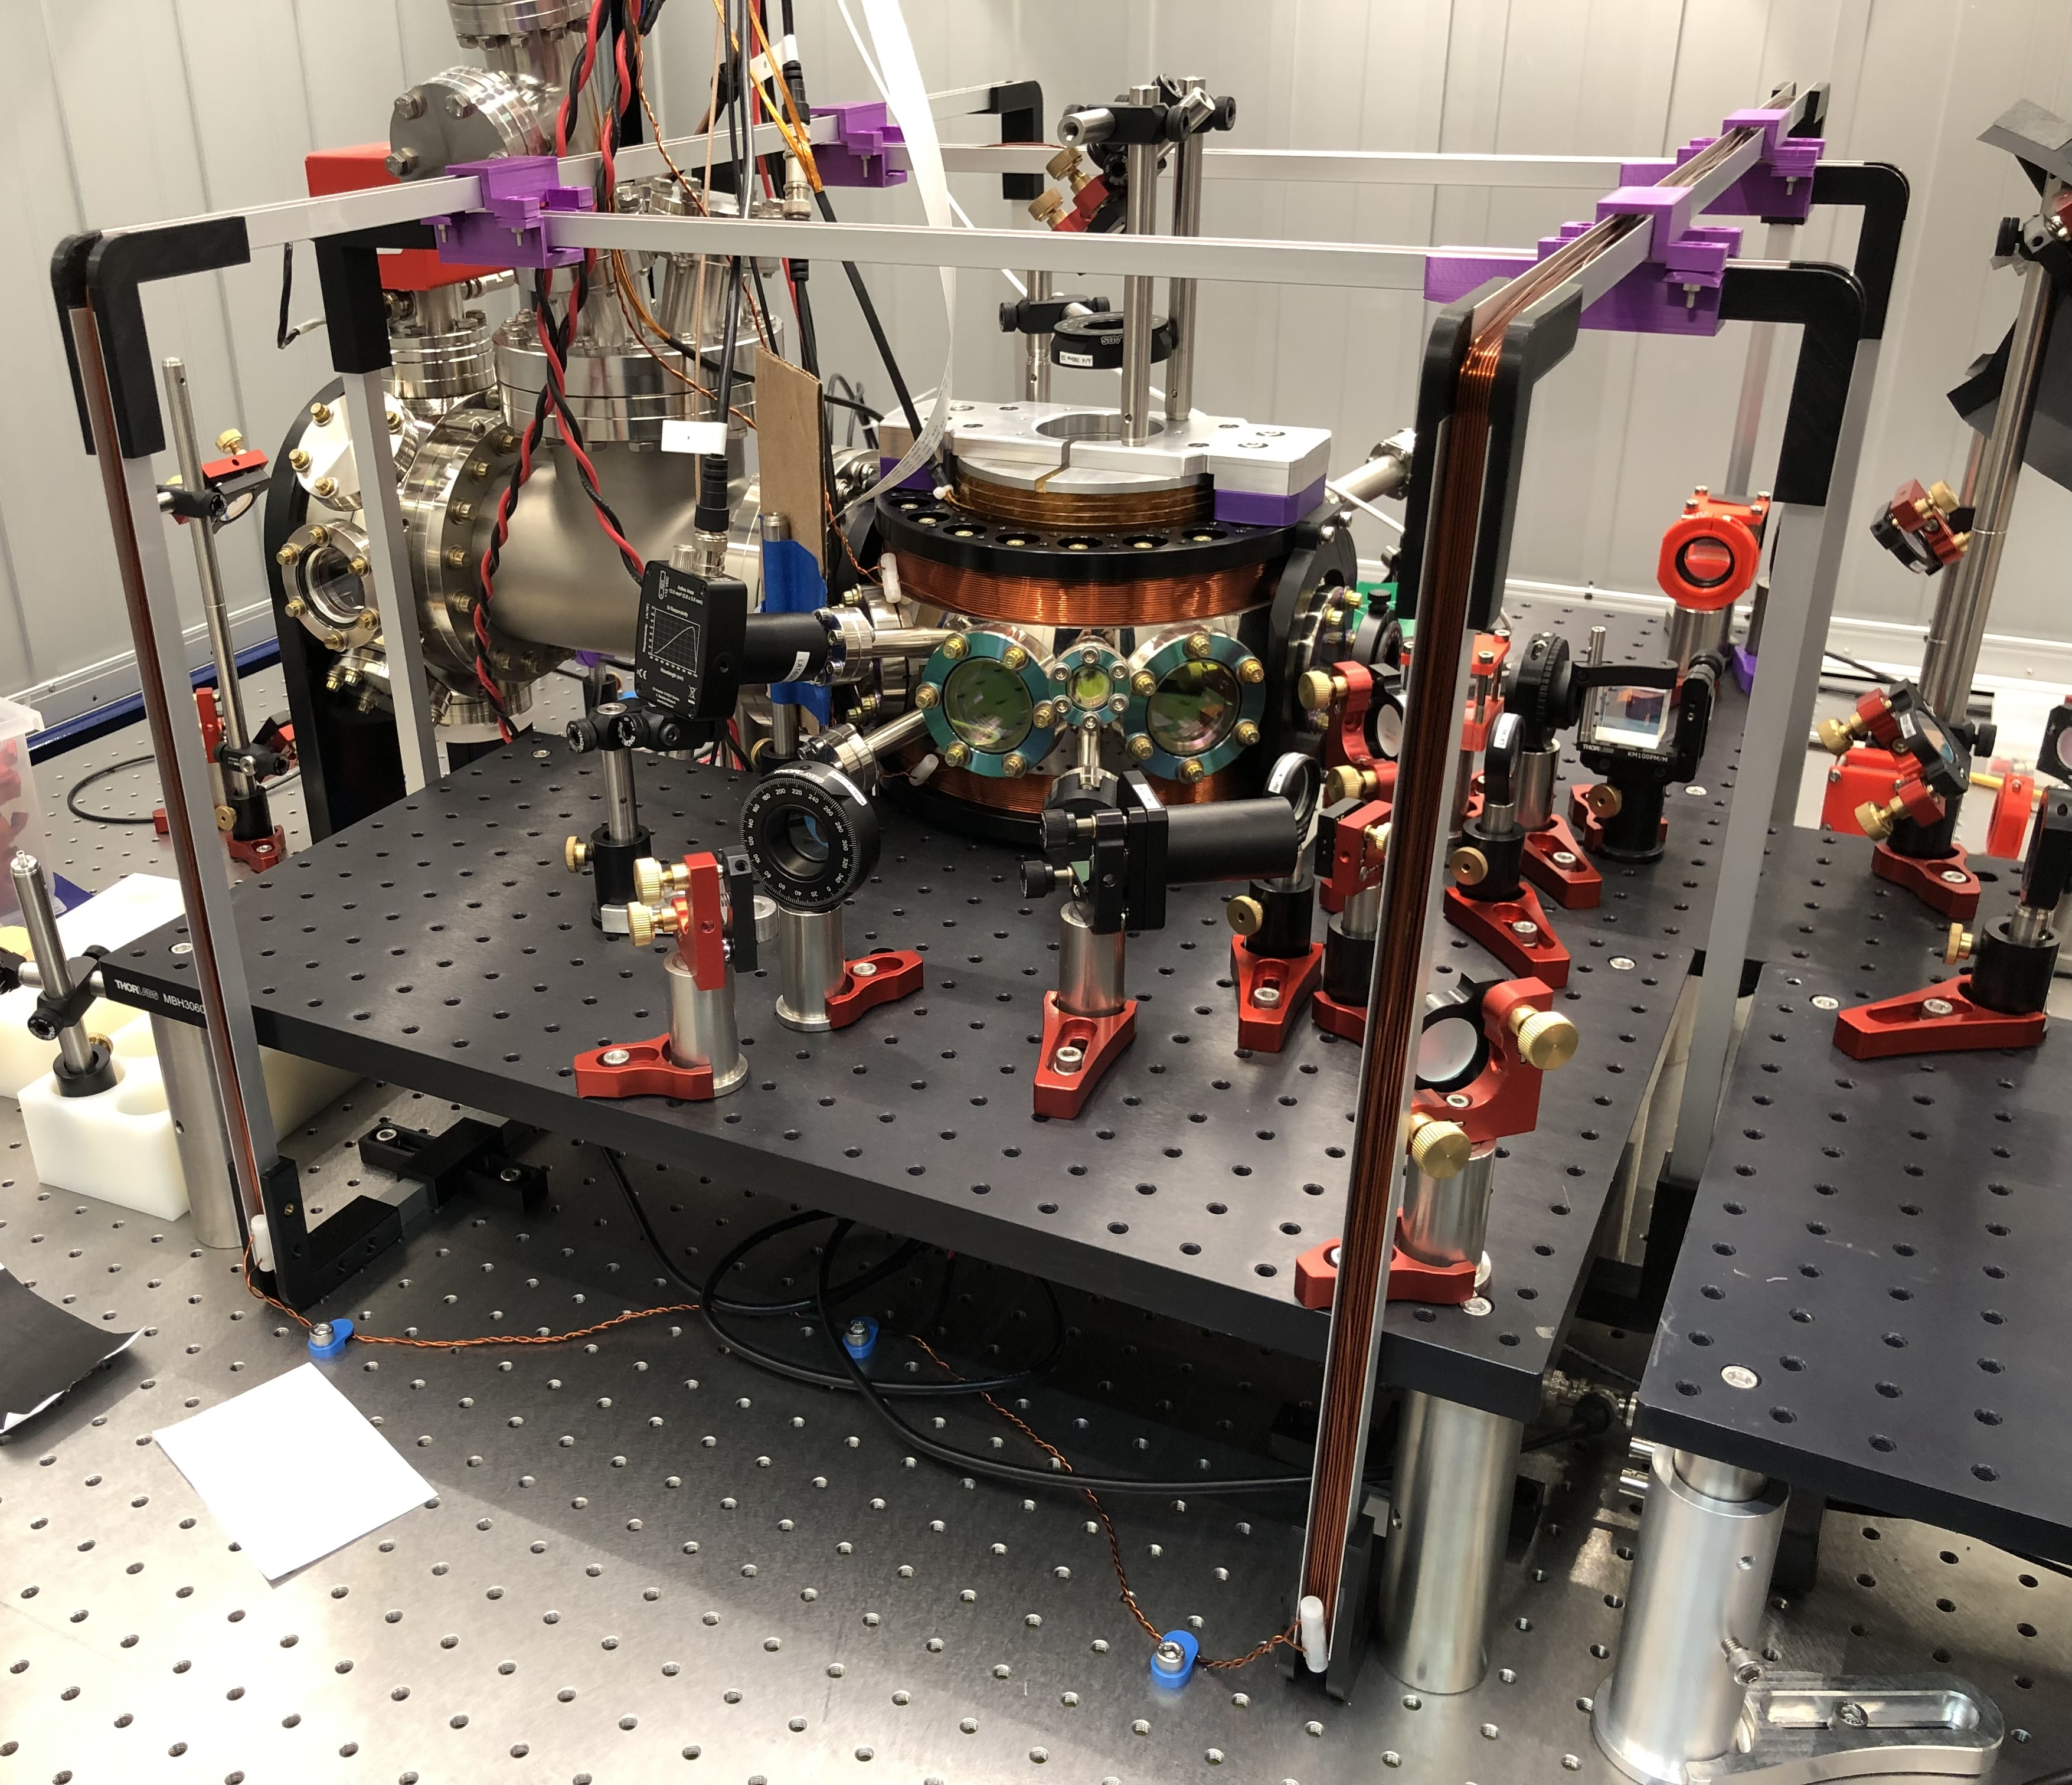
\includegraphics[width=0.4\linewidth]{bobinasBombeoOptico}}
\subcaptionbox{\label{fig:fotoExp}}[0.55\linewidth]{\usebox{\bobinasBox}}
\hfill
\subcaptionbox{\label{fig:bobinasBombeoOpticoDestacado}}[0.4\linewidth]{
\vbox to \ht\bobinasBox{
\vfill
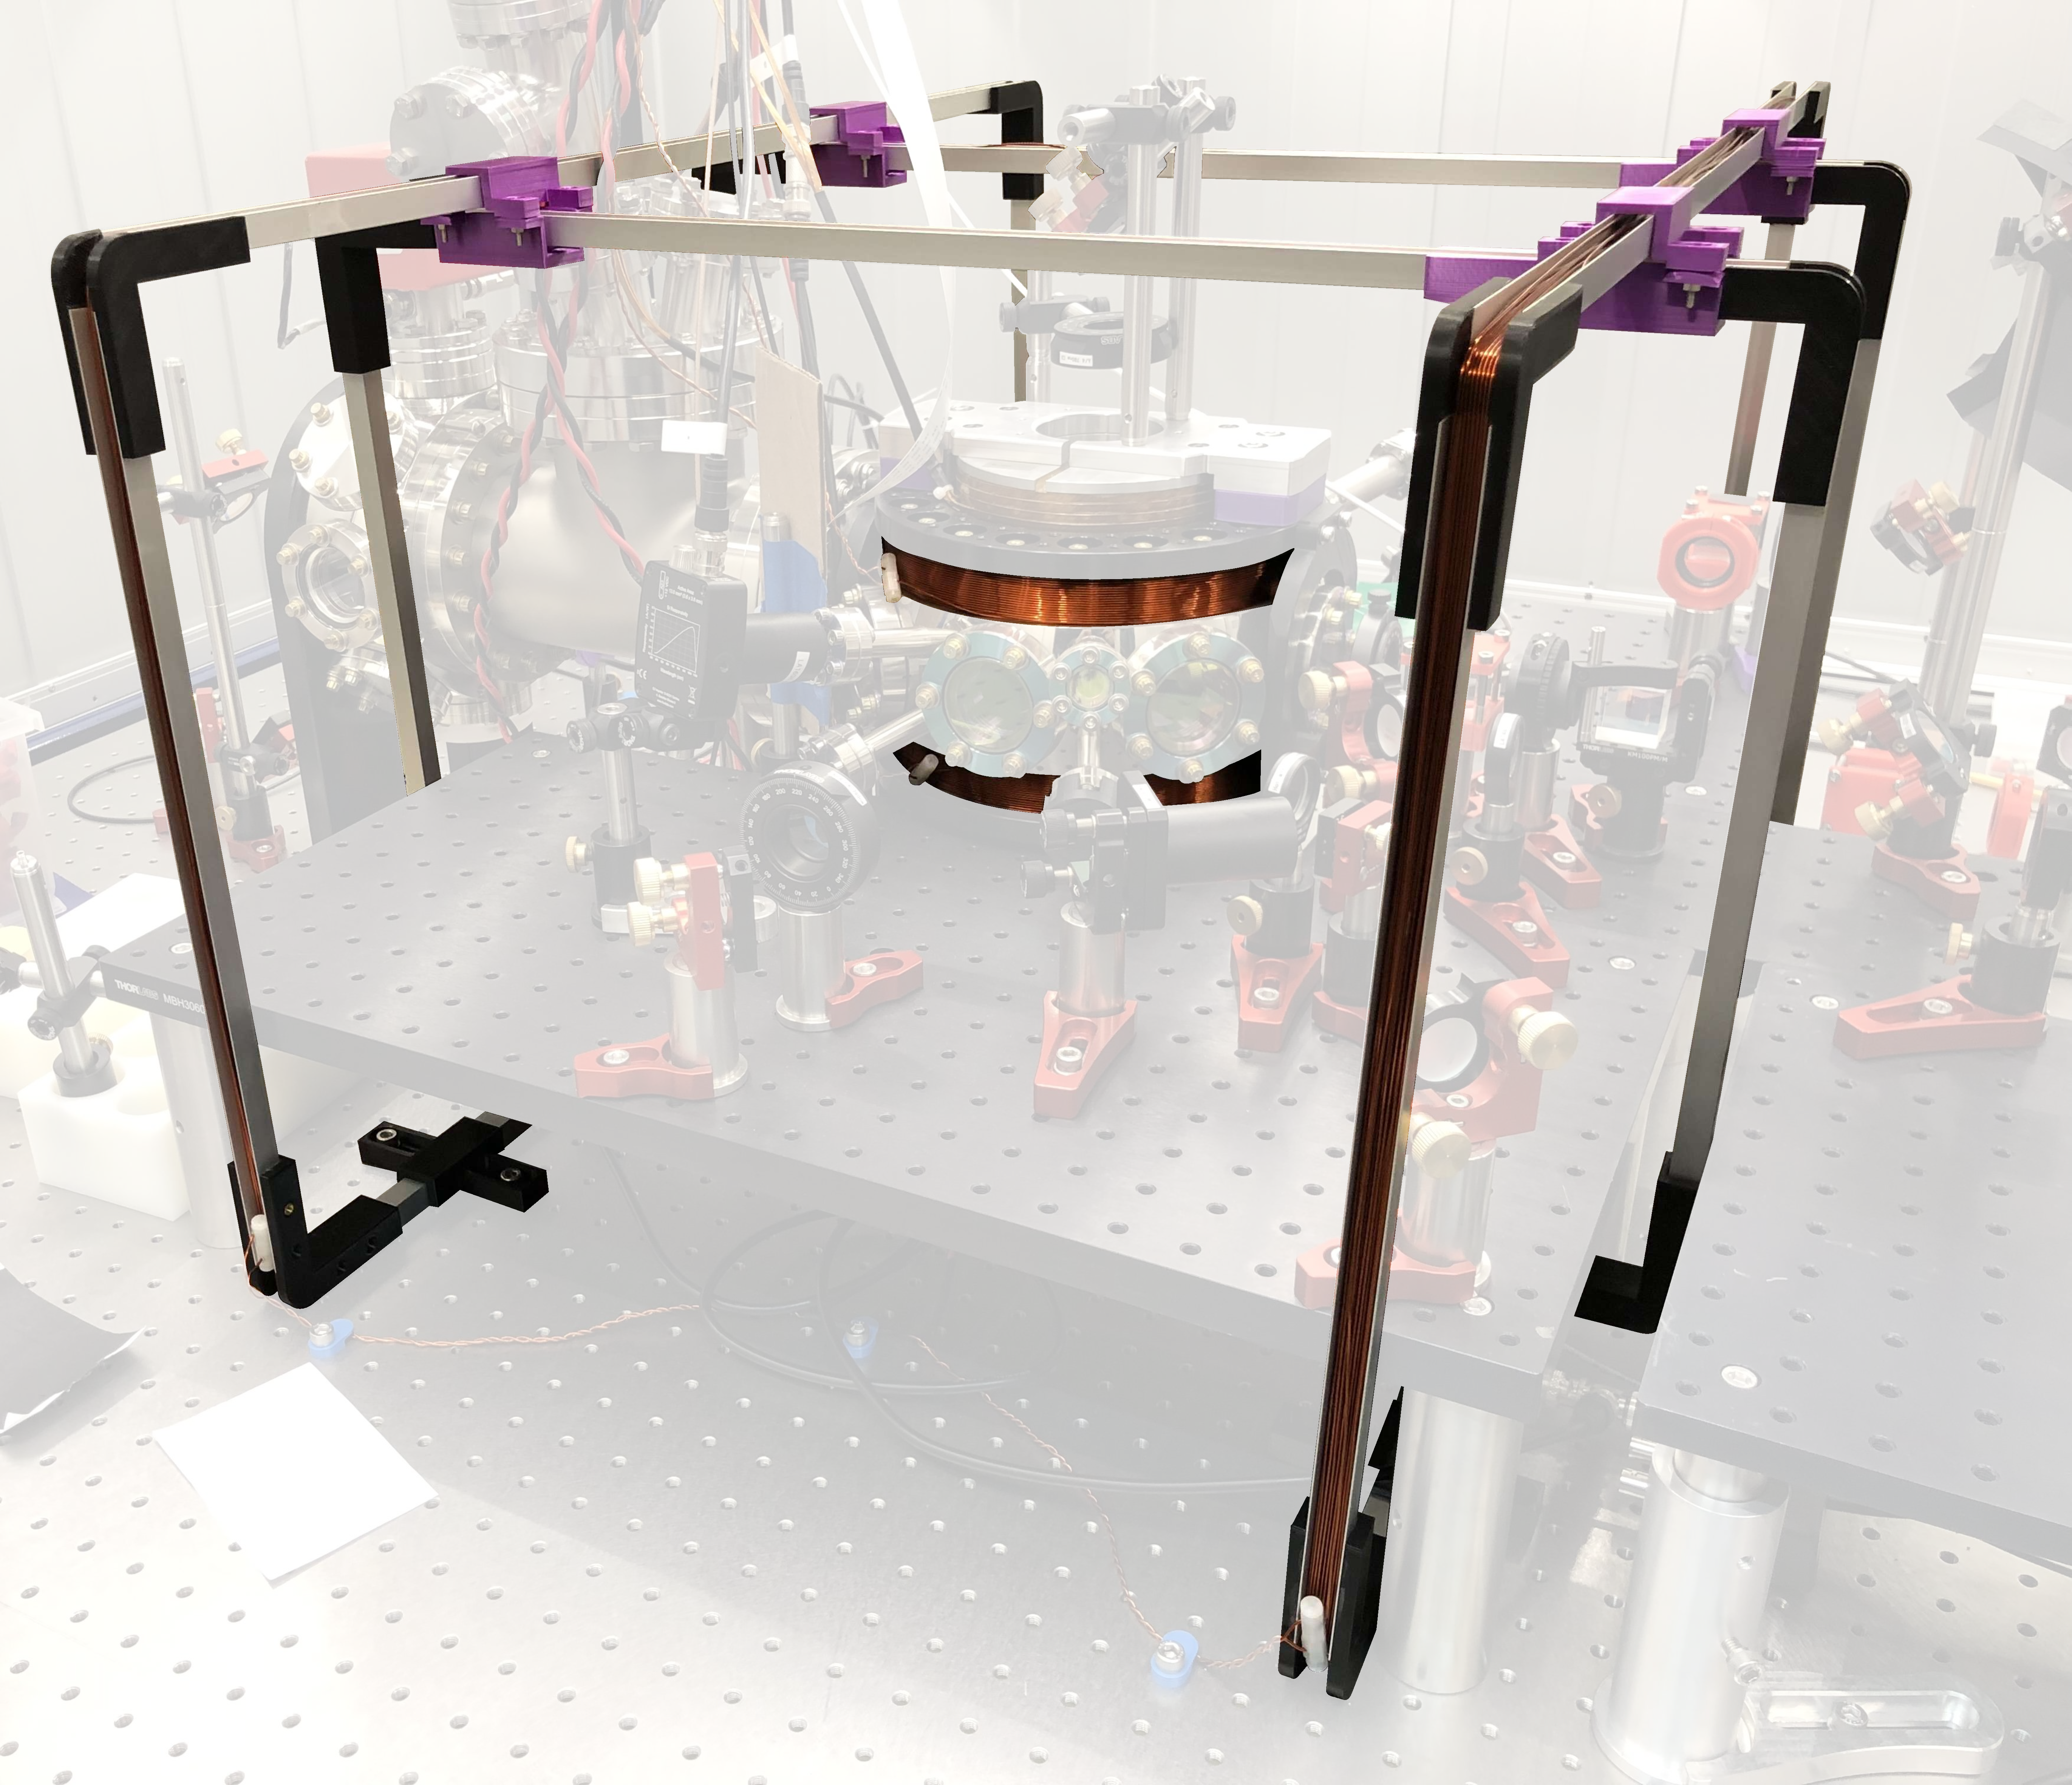
\includegraphics[width=\linewidth]{bobinasBombeoOpticoDestacado}
\vfill}}
\caption[Bobinas del Bombeo Óptico]{\label{fig:bobinasBombeoOptico}(a) Fotografía del sistema de vacío con parte de la optomecánica para formar los haces de la MOT. (b) Imagen donde se resaltan las bobinas del bombeo óptico. Los tres pares de bobinas son ortogonales entre sí.}
\end{minipage}
\end{figure}

Entonces, el campo constante de las bobinas del bombeo óptico nos deja ajustar el cero del campo de atrapamiento para empatarlo con los haces de la MOT, de esta manera el enfriamiento se hace con mayor eficiencia. En adición a las bobinas, usamos otro proceso de enfriamiento independiente de la MOT: una vez ha transcurrido el tiempo característico de carga de la MOT, desintonizamos la luz de los haces de enfriamiento todavía más hacia el rojo y disminuimos su potencia con una rampa de $\SI{1}{\milli\second}$ de duración. La combinación de este proceso con el ajuste del campo nos permite obtener nubes de átomos con temperaturas alrededor de los $\SI{10}{\micro\kelvin}$, un orden de magnitud mejor a situaciones previas.

\section{\label{sec:medicionesEIT}Mediciones de EIT}

Otro avance en el laboratorio fue la generación de la ventana de transparencia en los átomos debido al fenómeno de EIT, la figura~\ref{fig:esquemaEIT} es un esquema del montaje que hay en el laboratorio para esta medición . Lo logramos con un estado de Rydberg $28\mathrm{S}_\sm{1/2}$ del $\prescript{87}{}{\mathrm{Rb}}$. Antes de iniciar mi doctorado ya habíamos logrado producir EIT en nuestra nube de Rb, en lugar de hacer una detección del perfil de intensidad con una cámara CCD (como lo hacíamos aún más antes) utilizamos un contador de fotones (en concreto un SPCM, por sus siglas en inglés) con el objetivo de mejorar la señal a ruido, es decir, en la detección lo que tenemos es un histograma con las cuentas de fotones que llegan al contador. La intensidad del haz de prueba tiene que ser del orden de los $\si{\pico\watt}$ para no quemar el SPCM, nosotros establecemos una media de un millón de fotones por segundo.

\begin{figure}
\centering
\begin{minipage}{0.8\textwidth}
\centering
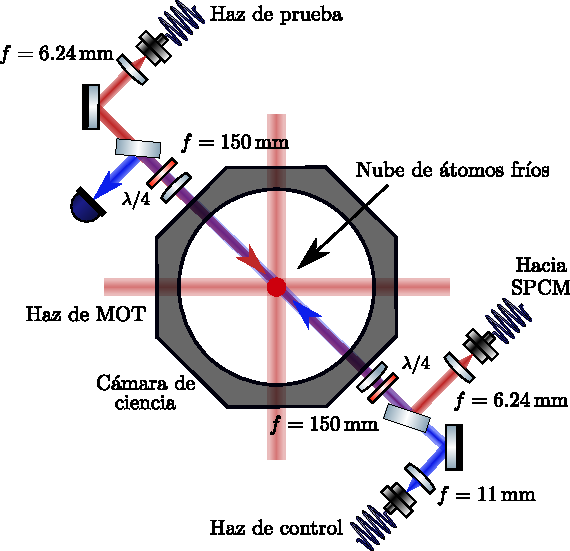
\includegraphics[width=0.8\textwidth]{esquemaEIT}
\caption{\label{fig:esquemaEIT}Esquema del montaje experimental con el que conseguimos excitaciones de Rydberg del Rb y la transparencia EIT. Los haces de prueba y de control son contrapropagantes y con intensidades muy diferentes, del orden de $\si{\pico\watt}$ la intensidad del láser de prueba y de $\si{\milli\watt}$ el haz de control.}
\end{minipage}
\end{figure}

\p El procedimiento que usamos para hacer mediciones del perfil EIT es el siguiente: se enfrían los átomos mediante la MOT para luego apagarla, dejando en caída libre la nube de átomos mientras se expande durante $\SI{100}{\micro\second}$. Inmediatamente después, y por $\SI{100}{\micro\second}$, prendemos la luz de prueba ($\delta_\sm{p}$) y de control (resonante) para realizar EIT, los fotones del láser de prueba que atraviesan el medio atómico son contabilizados por el SPCM. Nuevamente, dejamos caer la nube y a los $\SI{20}{\milli\second}$ volvemos a prender los haces para medir el número de fotones que pasan en ausencia de los átomos. El cociente de estas medidas nos da la transmitancia asociada al medio para la desintonía $\delta_\sm{p}$ del haz de prueba elegido, al repetir las mediciones para diferentes desintonías obtenemos el perfil de absorción de la nube.

\section{\label{sec:cambiadorFase}Cambiador de fase con dispositivos acusto-ópticos}

Dados los objetivos experimentales del laboratorio de OCR necesitamos controlar de forma muy precisa la fase de la luz: no sólo queremos producir estados no clásicos de luz, también queremos caracterizarlos y reconstruirlos a partir de las mediciones que realicemos. Con esto en mente se ideo un dispositivo para controlar la fase de la luz modulando su frecuencia, la razón detrás de esto es la precisión que tenemos en conocer y cambiar frecuencias. Llevamos a cabo el montaje y realización experimental con este susodicho dispositivo, el análisis de los resultados para cambiar la fase y la originalidad de hacerlo con aparatos acusto-ópticos resulto en su publicación en mayo de este año, con el título \emph{High-precision frequency-controlled optical phase shifter with acousto-optic devices}~\cite{esquivel}.

\p Nuestro dispositivo es, en esencia, un interferómetro Mach-Zehnder, la diferencia es que en lugar de modificar activamente la fase de la luz en uno de los brazos, introduciendo un objeto para modificar el camino óptico, cambiamos la frecuencia de uno de los brazos. Durante su propagación la fase relativa entre ambos brazos cambia gracias a que tienen frecuencias diferentes, y justo antes de la detección las frecuencias se vuelven a igualar para que interfieran los haces.

\begin{figure}
\centering
\begin{minipage}{0.8\textwidth}
\centering
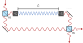
\includegraphics[width=0.8\textwidth]{principioFuncionamiento}
\caption{\label{fig:principioFuncionamiento}Principio de funcionamiento del cambiador de fase. Un haz láser pasa por un divisor de haz 50/50 (BS, por sus siglas en inglés). Uno de los brazos del interferómetro se propaga una distancia $L$ con un cambio de frecuencia sintonizable $f_\sm{S}$. El resultado es un cambio de fase efectivo con respecto al brazo que conserva la frecuencia inicial. Al final se recombinan con otro BS para analizar el cambio de fase mediante el cambio en el patrón de interferencia.}
\end{minipage}
\end{figure}

\p La figura~\ref{fig:principioFuncionamiento} esquematiza el funcionamiento de nuestro dispositivo. Usamos un divisor de haz para crear ambos brazos del interferómetro, la luz de uno de los brazos viaja una distancia $L$ con la frecuencia modificada, luego se regresa a su frecuencia inicial y con otro divisor de haz se recombinan los haces. La distancia $L$ está fija, sin embargo, al cambiar la frecuencia también lo hace el número de longitudes de onda que caben en $L$, esto deriva en una fase extra $\phi=2\pi n_\sm{r}Lf_\sm{S}/c$ con $f_\sm{S}$ la frecuencia que se añadió. El cambio de fase con esta técnica es proporcional al cambio de frecuencia.

\p Con este dispositivo podre realizar el análisis del cambio de fase de la luz que pasa por un medio en condiciones de EIT (ver~\ref{cap:plan}) así como medir cuadraturas del campo electromagnético para la reconstrucción de estados no clásicos de la luz.

\section{\label{sec:retrasoLuz}Medición del retraso de la luz}

Ya hemos realizado experimentos en condiciones de EIT para medir el retraso de la luz, sin embargo, utilizamos pulsos de luz con un perfil temporal cuadrado y no fuimos capaces de resolver si había o no retraso. Hasta ahora se ha desarrollado el programa para que un generador de funciones nos proporcione pulsos con perfil temporal gaussiano.